% !TeX root = ../../main.tex
\section{Corporate overview}
\subsection{Selection of location}
\label{app:location}

\begin{table}[H]
\centering
    \caption{AHP/TOPSIS results for plant location selection}
    \label{tab:location-selection}
\adjustbox{max width=\textwidth}{
\begin{tabular}{@{}l|ll|lll|ll|lll|l|l|llc@{}}
%S[table-format=2.2]S[table-format=1.2]S[table-format=1.3]
\toprule
                                          & \multicolumn{2}{c|}{\splitcell{Local supply chain\\ (\SI{34}{\percent})}}                               & \multicolumn{3}{c|}{\splitcell{Country economics\\ (\SI{17}{\percent})}} & \multicolumn{2}{c|}{\splitcell{Trade\\ (\SI{4}{\percent})}}     & \multicolumn{3}{c|}{Operating costs (\SI{28}{\percent})}   & \splitcell{Competitive\\ Landscape (\SI{9}{\percent})} & \splitcell{Political\\ stability (\SI{7}{\percent})}  &     &                      \\ \cmidrule{2-13}
                                          
                                      & {\rcell{Toluene production (\si{\kilo\tonne\per\year})}} & {\rcell{Market size of products (\si[prefixes-as-symbols=false]{\giga\USD})}} & \rtext{Interest rate (\%)}  & \rcell{Corporate tax rate (\%)} & \rtext{Inflation (\%)} & \rtext{Import duties (\%)} & \rtext{Export duties (\%)} & {\rcell{Electricity cost (\si{\USD\per\kWh})}} & {\rcell{Minimum wage (\si{\USD\per\hour})}} & {\rcell{Cooling water cost (\si{\USD\per\l})}} &  {\rcell{Number competitors}} & {\rcell{Corruption perception index}} & AHP & TOPSIS & Rank \\ \midrule
India & 923       & 20 & 4.00     & 30       &  7.35          &     4.9      & 7.50 & 0.08 & 1.00 & 0.20 & 2                 & 41                & 0.193 & 0.536 &    3              \\ 
China & 4314          & 95 & 3.85  & 15     &       1.60     & 3.4           & 6.50 & 0.08 & 1.68 & 0.33 & 48                 & 41                 & 0.284 & 0.922 & \cellcolor{green}1  \\ 
USA     & 4992        & 501  & 0.25      & 21      &     1.20        & 1.6    & 5.25 & 0.15 & 7.30 & 1.53       & 157               & 69                 & 0.218 & 0.659 & 2 \\ 
Germany      & 930            & 47 & 0.00   & 30      & -0.30            & 1.7      & 6.50 & 0.38 & 10.97 & 2.46     & 33               & 80                   & 0.182         & 0.485 &  4          \\ 
Poland    & 285           & 7.9 & 0.10      &   19   & 12.60            & 2.5 & 6.50 & 0.19 & 3.35 & 0.93         & 0                 & 39                  &    0.123         & 0.290 &     5      \\ 
\bottomrule
\end{tabular}
} % adjustbox
\end{table}

\subsection{Results of Porter's Five Forces analysis}
\label{app:five-forces}

\label{sec:business-timeline}
\begin{figure}[h]
\centering
 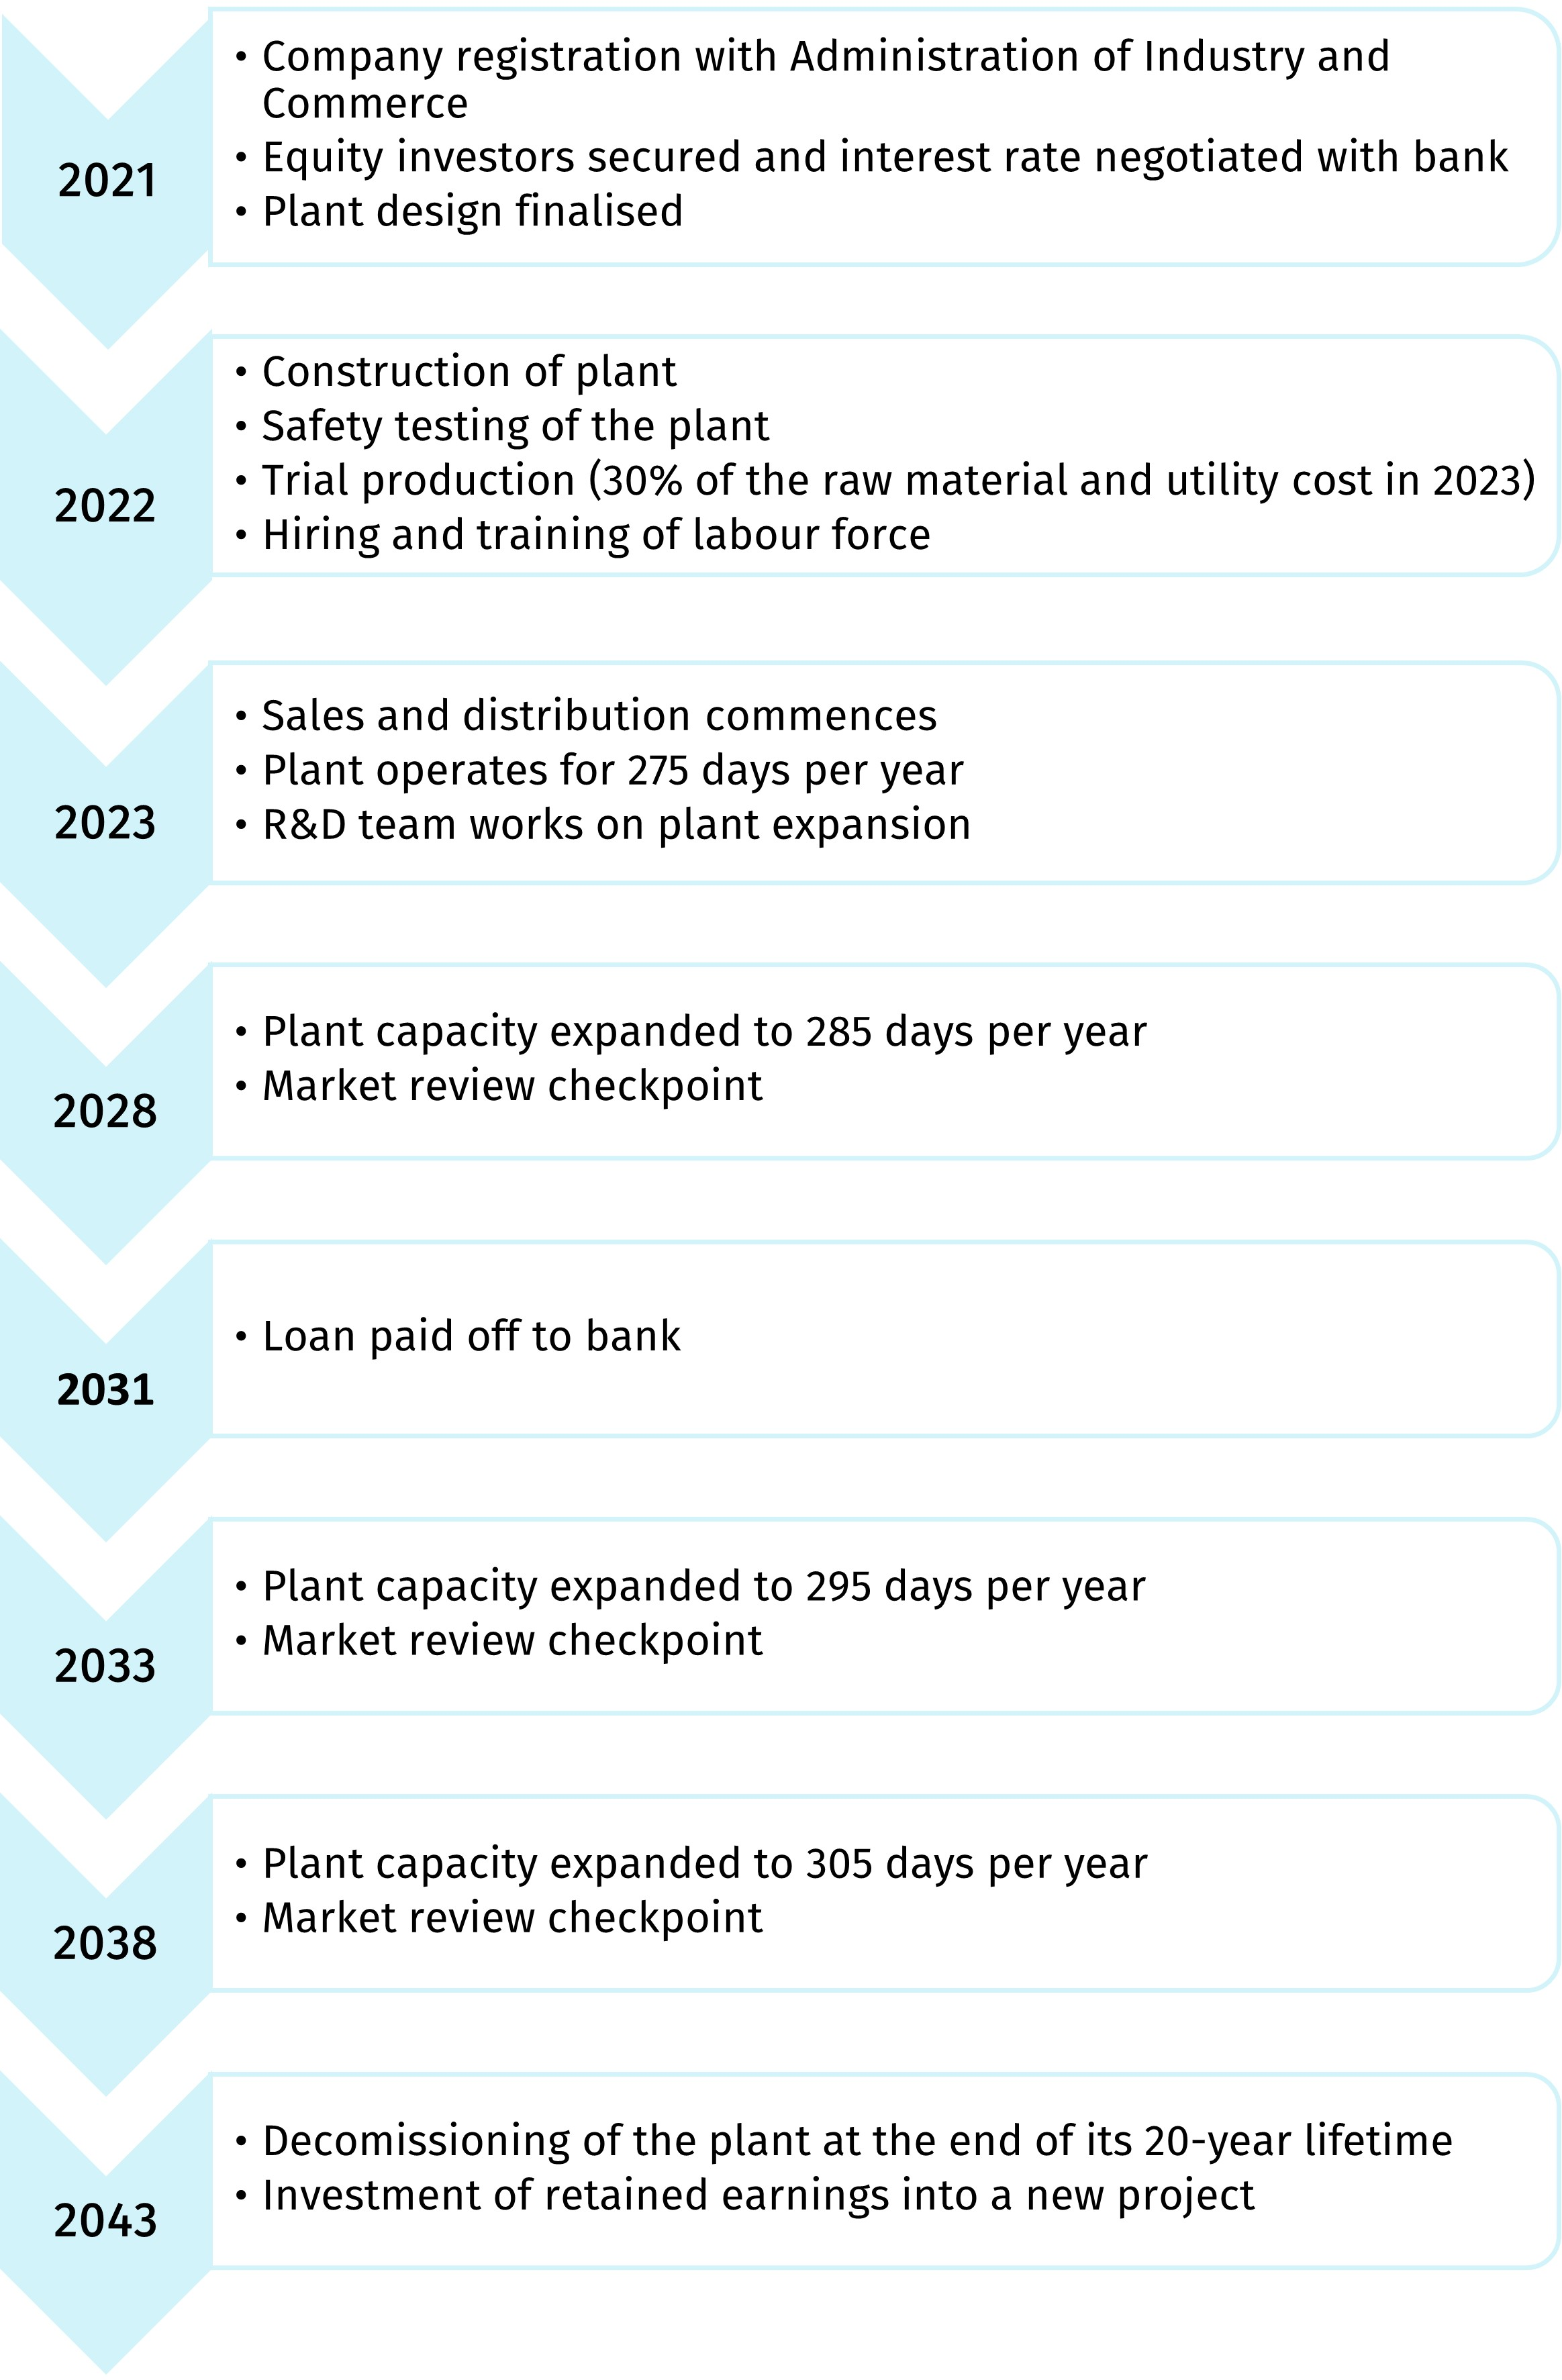
\includegraphics[width=12.5cm]{chapters/6-economics/figures/Business timeline.jpg}
 \caption{Nitroma's business timeline}
 \label{fig:business-timeline}
\end{figure}

\subsection{SWOT results}

\begin{table}[h]
    \centering
    \caption{SWOT analysis}
    \label{tab:swot}
    
    \begin{tabularx}{\linewidth}{l|X|X}
        & \textit{Helpful} & \textit{Harmful} \\ \hline
        \rotatebox[origin=r]{90}{\textit{Internal}} & \begin{minipage}[t]{\linewidth} \makebox[\linewidth]{\color{green}\textbf{Strengths}}
        \begin{itemize}[topsep=0em,leftmargin=1em]
            \item hello
        \end{itemize}\end{minipage} & \begin{minipage}[t]{\linewidth} \makebox[\linewidth]{\color{yellow}\textbf{Weaknesses}}
        \begin{itemize}[topsep=0em,leftmargin=1em]
            \item world
        \end{itemize}\end{minipage} \\ \hline 
        \rotatebox[origin=r]{90}{\textit{External}} & \begin{minipage}[t]{\linewidth} \makebox[\linewidth]{\color{blue}\textbf{Opportunities}} 
        \begin{itemize}[topsep=0em,leftmargin=1em]
            \item foo
        \end{itemize}\end{minipage} & \begin{minipage}[t]{\linewidth} \makebox[\linewidth]{\color{red}\textbf{Threats}}
        \begin{itemize}[topsep=0em,leftmargin=1em]
            \item bar
        \end{itemize}\end{minipage} \\
    \end{tabularx}
    
\end{table}